\documentclass[10pt, aspectratio=169]{beamer}
%\documentclass[handout,....]{beamer}  to get rid of \pause slides!

\setbeamertemplate{frametitle}[default][center]
\setbeamertemplate{navigation symbols}{}
\setbeamertemplate{footline}[frame number]
\setbeamertemplate{itemize items}[circle]

\setbeamercolor{block body alerted}{bg=alerted text.fg!10}
\setbeamercolor{block title alerted}{bg=alerted text.fg!20}
\setbeamercolor{block body}{bg=structure!10}
\setbeamercolor{block title}{bg=structure!20}
\setbeamercolor{block body example}{bg=green!10}
\setbeamercolor{block title example}{bg=green!20}
\setbeamertemplate{blocks}[rounded]%[shadow]

\makeatletter
\def\blfootnote{\xdef\@thefnmark{}\@footnotetext}
\makeatother

\usepackage{tikz}
\usepackage[export]{adjustbox}

\title{Journal Club}
\author{Valentin Marteau}
\date{31.05.2022}

\begin{document}
{
 \usebackgroundtemplate{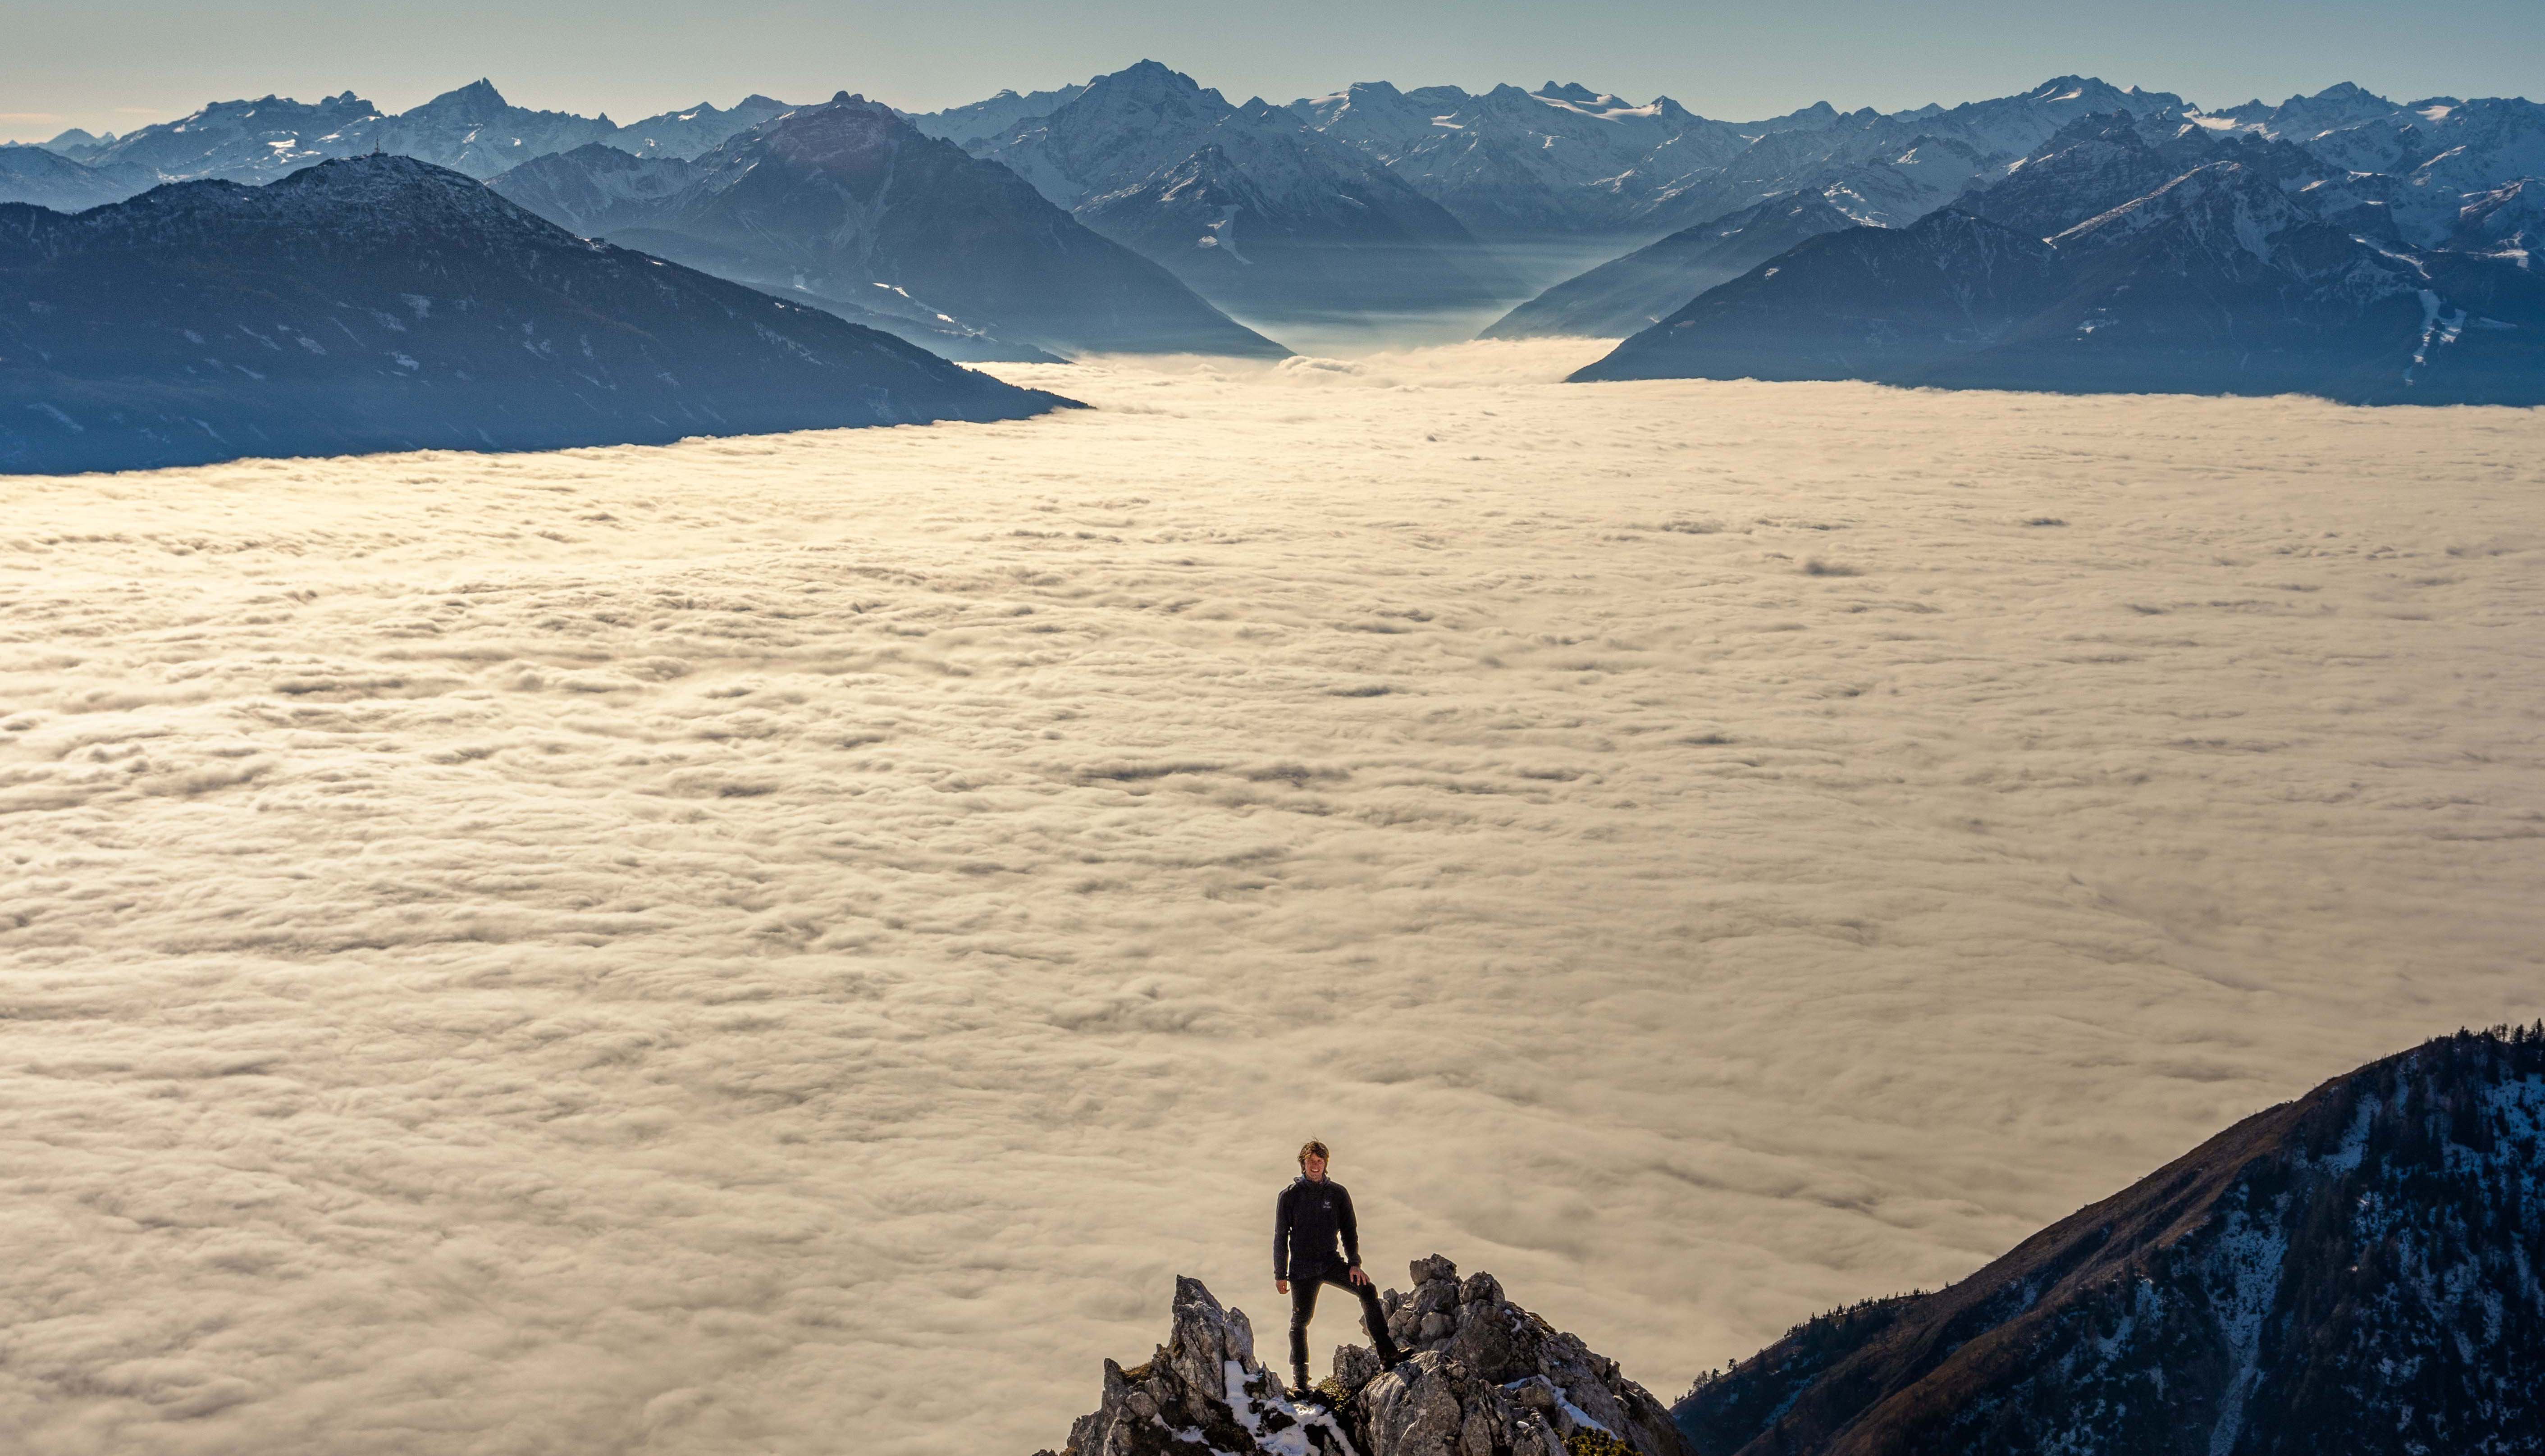
\includegraphics[width=\paperwidth]{figures/VJM_3542.jpg}}
  \begin{frame}
    \titlepage
  \end{frame}
}

\begin{frame}{Paper}
\centering
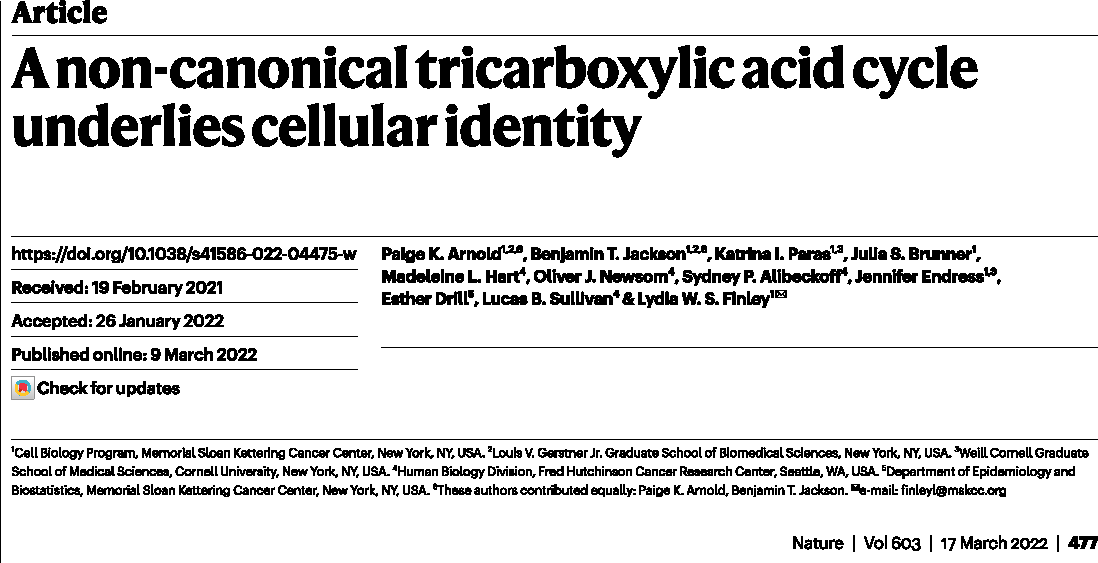
\includegraphics[width=0.9\textwidth]{figures/Arnold_2022_title.pdf}
\end{frame}

\begin{frame}{Aim}
\begin{columns}
\column{0.7\linewidth}

\begin{block}{\centering Tricarboxylic acid (TCA) cycle:}
\vspace{0.2cm}
    \begin{itemize}
        \item Central hub of cellular metabolism imortant for both energy production and biosynthesis \\[0.2cm]
        \item Series of chemical reactions to release stored energy through the oxidation of acetyl-CoA derived from carbohydrates, fats, and proteins\\[0.2cm]
        \item Mammalian cells display diversity in TCA-cycle activity \\[0.2cm]
    \end{itemize}
\vspace{0.2cm}
\end{block}

%TCA cycle is a hub of metabolism, with central importance in both energy production and biosynthesis
\vspace{0.3cm}

\pause
\begin{itemize}
    \item[$\rightarrow$] \textbf{How is this diversity achieved?} \\[0.3cm]
    \item[$\rightarrow$] \textbf{Is the TCA cycle critical for establishing cell fate?}
\end{itemize}

\column{0.3\linewidth}
\onslide
\centering
\includegraphics[width=0.9\textwidth]{figures/Martínez-Reyes_2020_fig2.pdf}\\[0.1cm]
\tiny{Martínez-Reyes \& Chandel; \textit{Nat. Commun.} (2020)}
\end{columns}
\end{frame}

\begin{frame}{DepMap project}

\begin{columns}			
\column{0.5\linewidth}

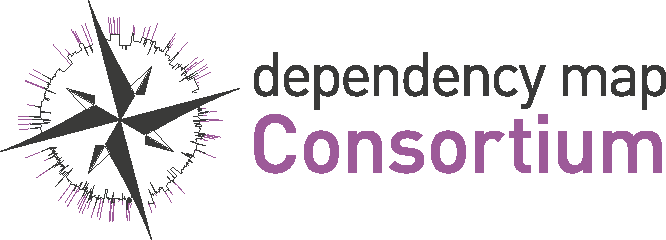
\includegraphics[width=0.8\textwidth,valign=t]{figures/depmap_consortium_logo.pdf}\\[0.3cm]
\begin{itemize}
    \item \textbf{Project goal:} Systematic identification of cancer dependencies \\[0.1cm]
    \item Genome-scale loss-of-function screens performed in diverse human cancer cell lines \\[0.1cm]
    \item Dependency score: Function of both the magnitude of the differential dependency and its prevalence in cell line collection
    
\end{itemize}

\column{0.5\linewidth}
\centering
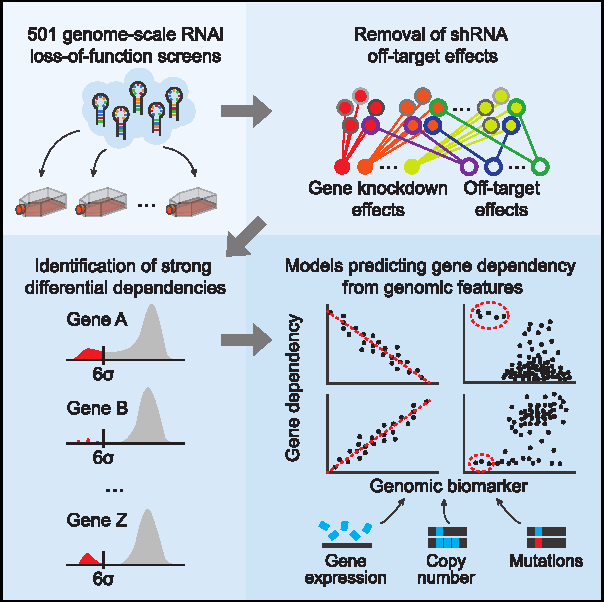
\includegraphics[width=0.95\textwidth]{figures/Tsherniak_2017_graphical_abstract.pdf}\\
\tiny{Tsherniak \textit{et al}. \textit{Cell} (2017)}

\end{columns}

\blfootnote{
\includegraphics[width=0.12\textwidth]{figures/depmap_consortium_logo2.pdf}}
\end{frame}

\begin{frame}{Metabolic gene essentiality correlations across cancer cell lines}
\centering
\includegraphics[width=0.74\textwidth]{figures/Arnold_2022_figS1.png}
\end{frame}

% How to use overlay options: https://www.overleaf.com/learn/latex/Beamer_Presentations%3A_A_Tutorial_for_Beginners_(Part_4)—Overlay_Specifications
\begin{frame}{Two modes of TCA cycle metabolism}

\uncover<1,2,3,4>{
\begin{figure}
\begin{tikzpicture}
\node[anchor=south west,inner sep=0] (image) at (4,0) {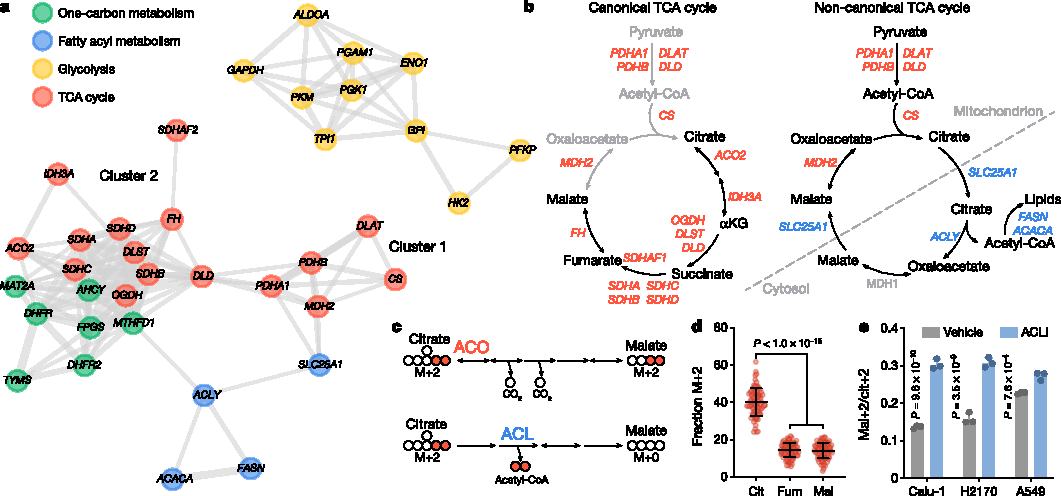
\includegraphics[width=0.98\textwidth]{figures/Arnold_2022_fig1.pdf}};
    \only<2>{%
        \fill [draw=none, fill=white, fill opacity=0.8] (image.north west) -- (image.north east) -- (image.south east) -- (image.south west) -- (image.north west) -- cycle;
\node[] at (image.center) {\vbox {\normalsize
    {\begin{block}{\centering Stable isotope tracing:}
    \vspace{0.2cm}
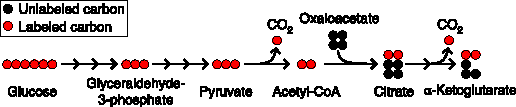
\includegraphics[width=\textwidth]{figures/Llufrio_2019_fig1.pdf}
\centering
\tiny{Llufrio, Cho \& Patti; \textit{Nature Protocols} (2019)}\\[0.2cm]
    \vspace{0.1cm}
    \end{block}
}
}};
}
\only<3>{}
\only<4>{%
        \fill [draw=none, fill=white, fill opacity=0.8] (image.north west) -- (image.north east) -- (image.south east) -- (image.south west) -- (image.north west) -- cycle;
\node[] at (image.center) {\vbox {\normalsize
    {\begin{block}{\centering Main points:}
    \vspace{0.2cm}
    \begin{itemize}
        \item Mapping gene cluster onto TCA cycle suggest clear division up-/downstream of citrate \\[0.3cm]
        \item \textbf{Hypothesis}: ACL may support metabolic demands by forming a non-canonical TCA cycle, capable of continuous oxaloacetate regeneration for citrate production \\[0.3cm]
        \item \textsuperscript{13}C labelled $\frac{malate}{citrate}$ ratio to monitor canonical vs. non-canonical TCA cycle activity
    \end{itemize}
    \vspace{0.3cm}
    \end{block}
\vspace{0.3cm}
    \begin{itemize}
    \centering
        \item[$\rightarrow$] \Large\textbf{What about non-transformed cells?}
    \end{itemize}}
}};
}

\end{tikzpicture}
\end{figure}
}
\blfootnote{ACO: aconitase; ACL: ATP citrate lyase}
\end{frame}

\begin{frame}{Embryonic stem (ES) cells engage a non-canonical TCA cycle}

\begin{columns}			
\column{0.5\linewidth}
\centering
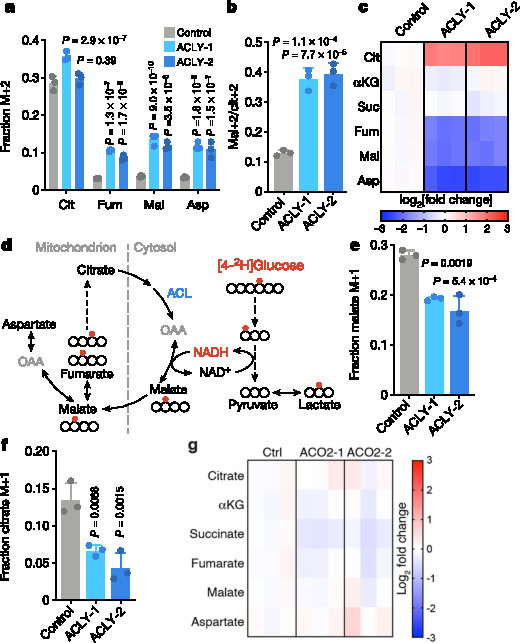
\includegraphics[width=0.85\textwidth]{figures/Arnold_2022_fig2_mod.pdf}

\column{0.6\linewidth}

\begin{itemize}
    \item ES cell line with genetic disruption of Acly and Aco2 \\[0.2cm]
    \item Acly mutation substantially alters levels of TCA cycle metabolites associated with cytosolic citrate processing\\[0.5cm]
    \pause
    \item[$\rightarrow$] Does a portion of the TCA cycle flow through ACL?\\[0.2cm]
    \pause
    \item Deuterated [4-\textsuperscript{2}H] glucose tracing\\[0.2cm]
    \pause
    \item \textbf{Cytosolic malate is recycled back into the mitochondria for citrate regeneration}
\end{itemize}
\end{columns}

\end{frame}


\begin{frame}{TCA cycle choice is cell-state dependent}
\begin{columns}			
\column{0.5\linewidth}
\centering
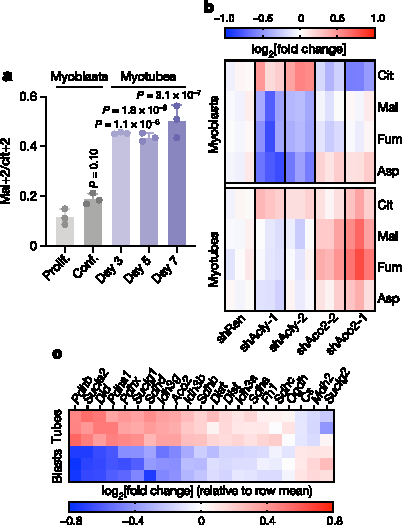
\includegraphics[width=0.8\textwidth]{figures/Arnold_2022_fig3_2.pdf}

\column{0.6\linewidth}

\begin{itemize}
    \item TCA cycle choice in myoblasts and differentiated myotubes \\[0.2cm]
    \item \textbf{Myotubes:} increased incorporation of glucose-derived carbons into TCA cycle intermediates\\[0.2cm]
    \item ACL inhibition effect stronger in myoblasts\\[0.2cm]
    \item ACO inhibition effect stronger in myotubes\\[0.5cm]
    \pause
    \item[$\rightarrow$] \textbf{When does the TCA cycle switch occur during differentiation?}
\end{itemize}

\end{columns}
\end{frame}

\begin{frame}{Exit from pluripotency requires ACL}
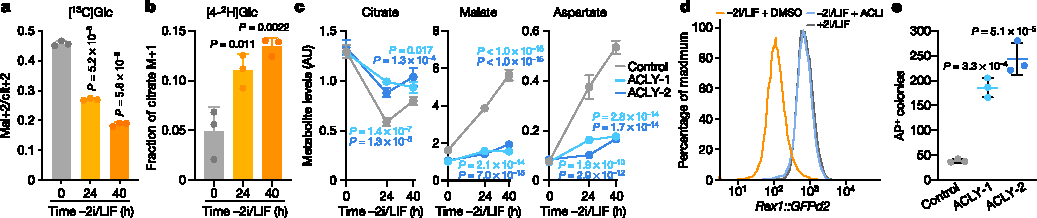
\includegraphics[width=\textwidth]{figures/Arnold_2022_fig4.pdf}

\vspace{0.3cm}

\begin{itemize}
    \item TCA cycle switch after pluripotency exit\\[0.2cm]
    \item Differentiated cells rely on the non-canonical TCA cycle to maintain TCA cycle intermediates\\[0.2cm]
    \item TCA cycle configuration plays a role in facilitating cell state transitions
\end{itemize}

\end{frame}

\begin{frame}{Summary}
\begin{itemize}
    \item[$\rightarrow$] Combining isotope tracing with genetic manipulation of Acly and Aco2 provide direct evidence of a non-canonical TCA cycle with differential activity across cell states\\[0.3cm]
\pause    
    \item[$\rightarrow$] \textbf{Main advantages:}
\begin{itemize}
    \item Retain rather than combust reduced carbon and regenerate cytosolic NAD\textsuperscript{+} required to sustain glycolysis\\[0.2cm]
    \item Non-canonical TCA cycle maintains oxaloacetate regeneration by circumventing several TCA cycle steps which minimizes mitochondrial NADH production \\[0.3cm]
\end{itemize}
\pause
    \item[$\rightarrow$] Starting hypothesis based on genetic co-essentiality mapping database \textbf{DepMap}
\end{itemize}
\end{frame}

\begin{frame}{Cancer Dependency Map}

\begin{columns}			
\column{0.6\linewidth}

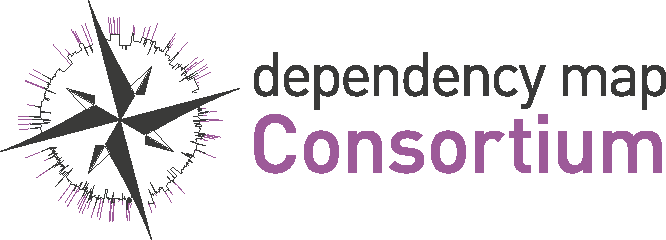
\includegraphics[width=0.8\textwidth]{figures/depmap_consortium_logo.pdf}\\[0.3cm]
\begin{itemize}
    \item \textbf{Project goal:} Systematic identification of genetic and pharmacologic cancer dependencies and the biomarkers that predict them
\end{itemize}

\column{0.5\linewidth}
\centering
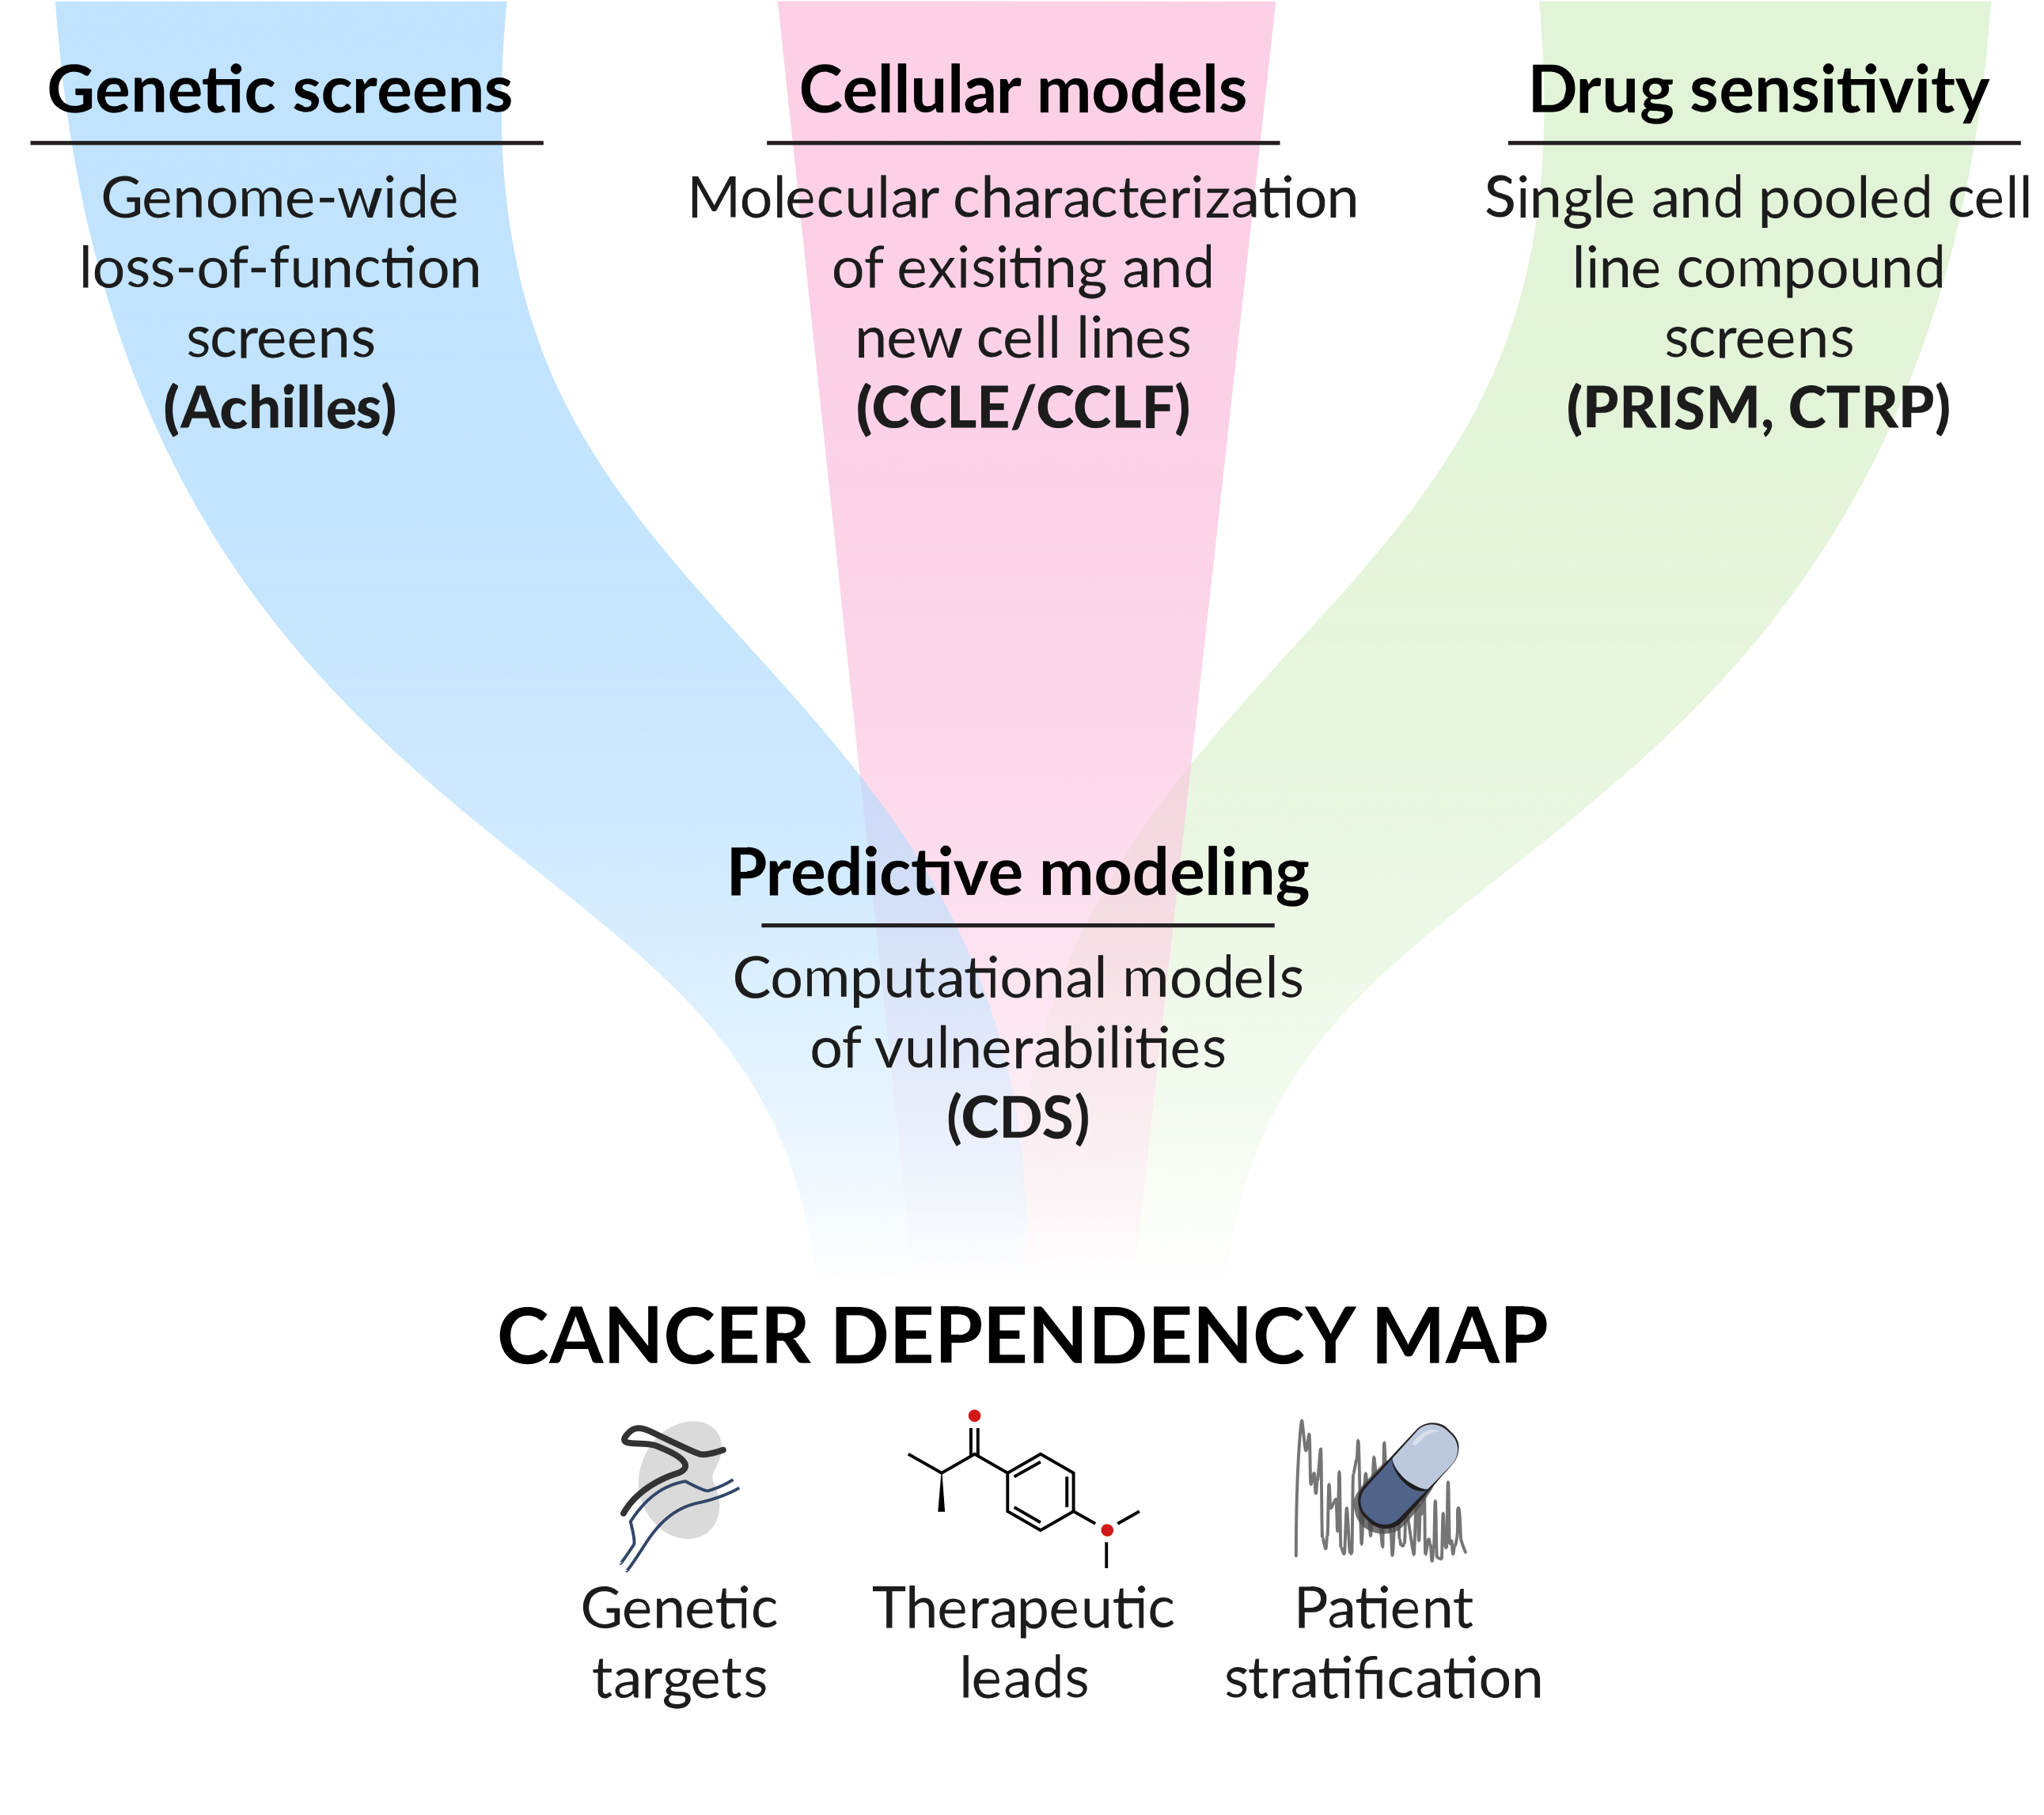
\includegraphics[width=\textwidth]{figures/depmapmodel.png}

\end{columns}

\blfootnote{
\includegraphics[width=0.12\textwidth]{figures/depmap_consortium_logo2.pdf}}
\end{frame}

\begin{frame}{Cancer Dependency Map}

\begin{columns}			
\column{0.6\linewidth}

\begin{itemize}
    \item Achilles project 22Q2 release: 17,387 genes were screened in 1086 cell lines \\[0.2cm]
    \item[$\rightarrow$] \textbf{R} Bioconductor package: "depmap" \\[0.2cm]
    \item[$\rightarrow$] \textbf{Python} PyPI package: "depmap-downloader"
\end{itemize}

\column{0.5\linewidth}
\centering
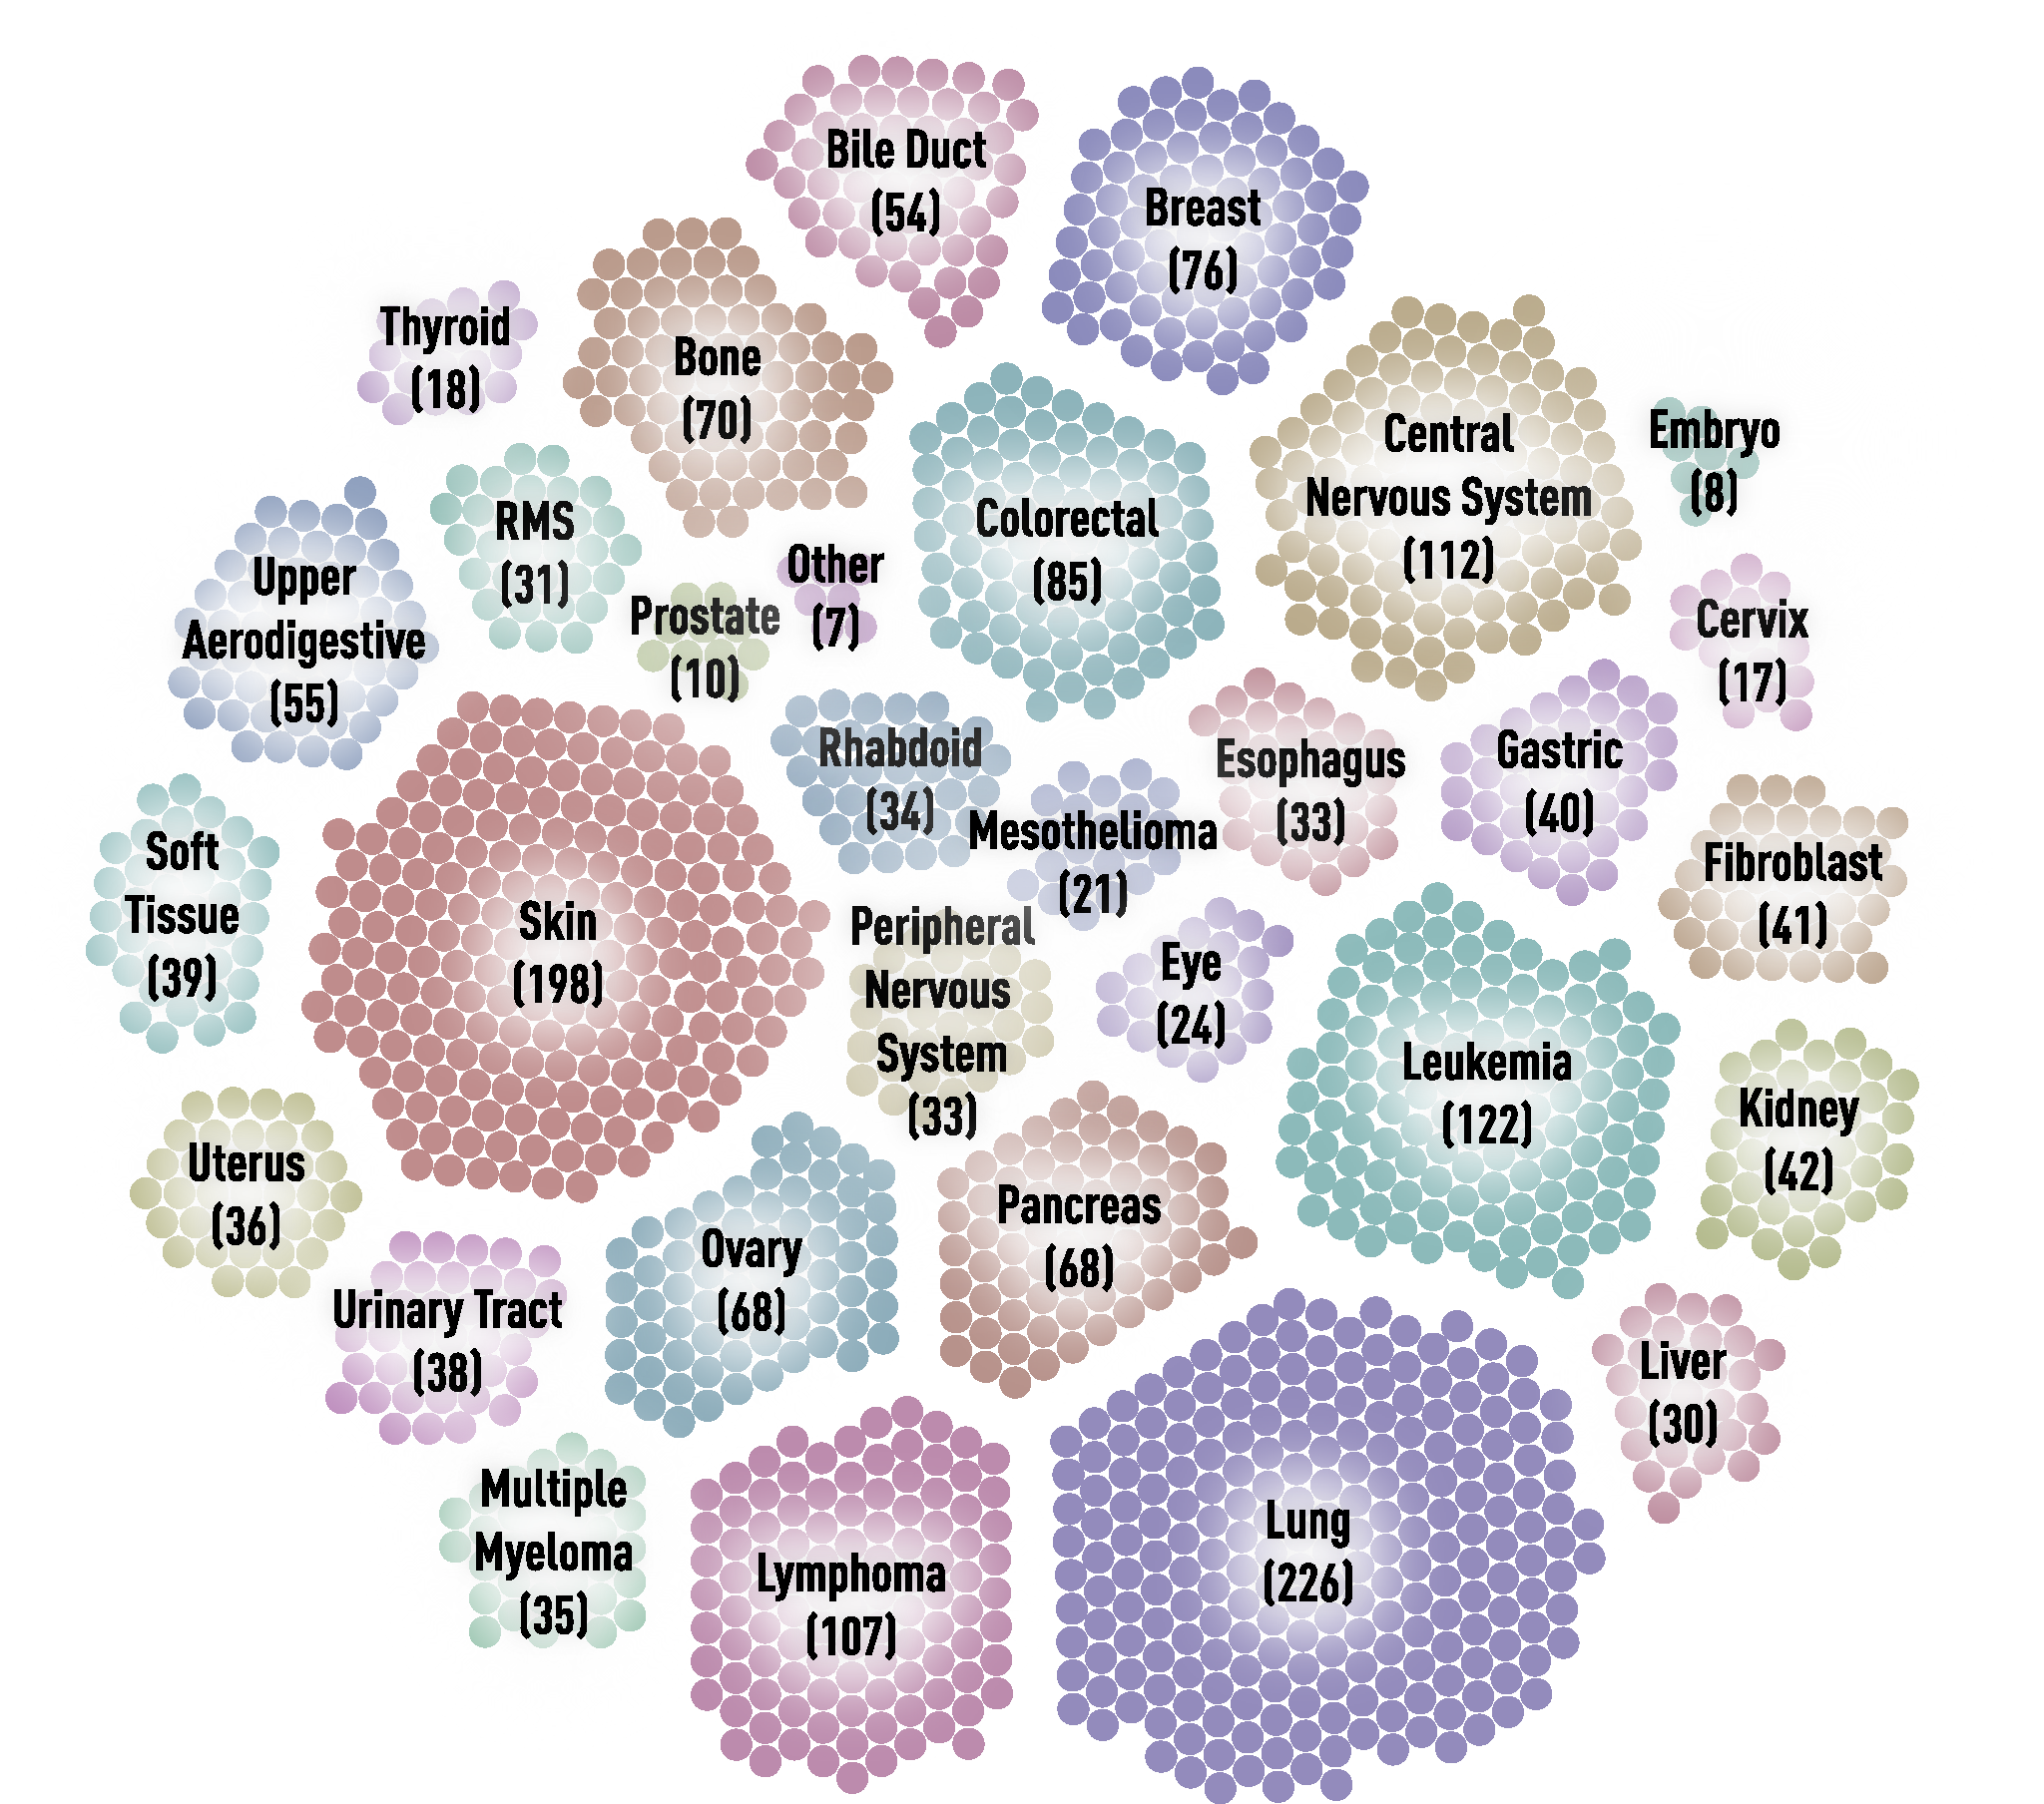
\includegraphics[width=0.95\textwidth]{figures/depmap_cell_lines_bubble_graph.pdf}

\end{columns}

\blfootnote{
\includegraphics[width=0.12\textwidth]{figures/depmap_consortium_logo2.pdf}}
\end{frame}

\begin{frame}{DepMap Data Explorer}
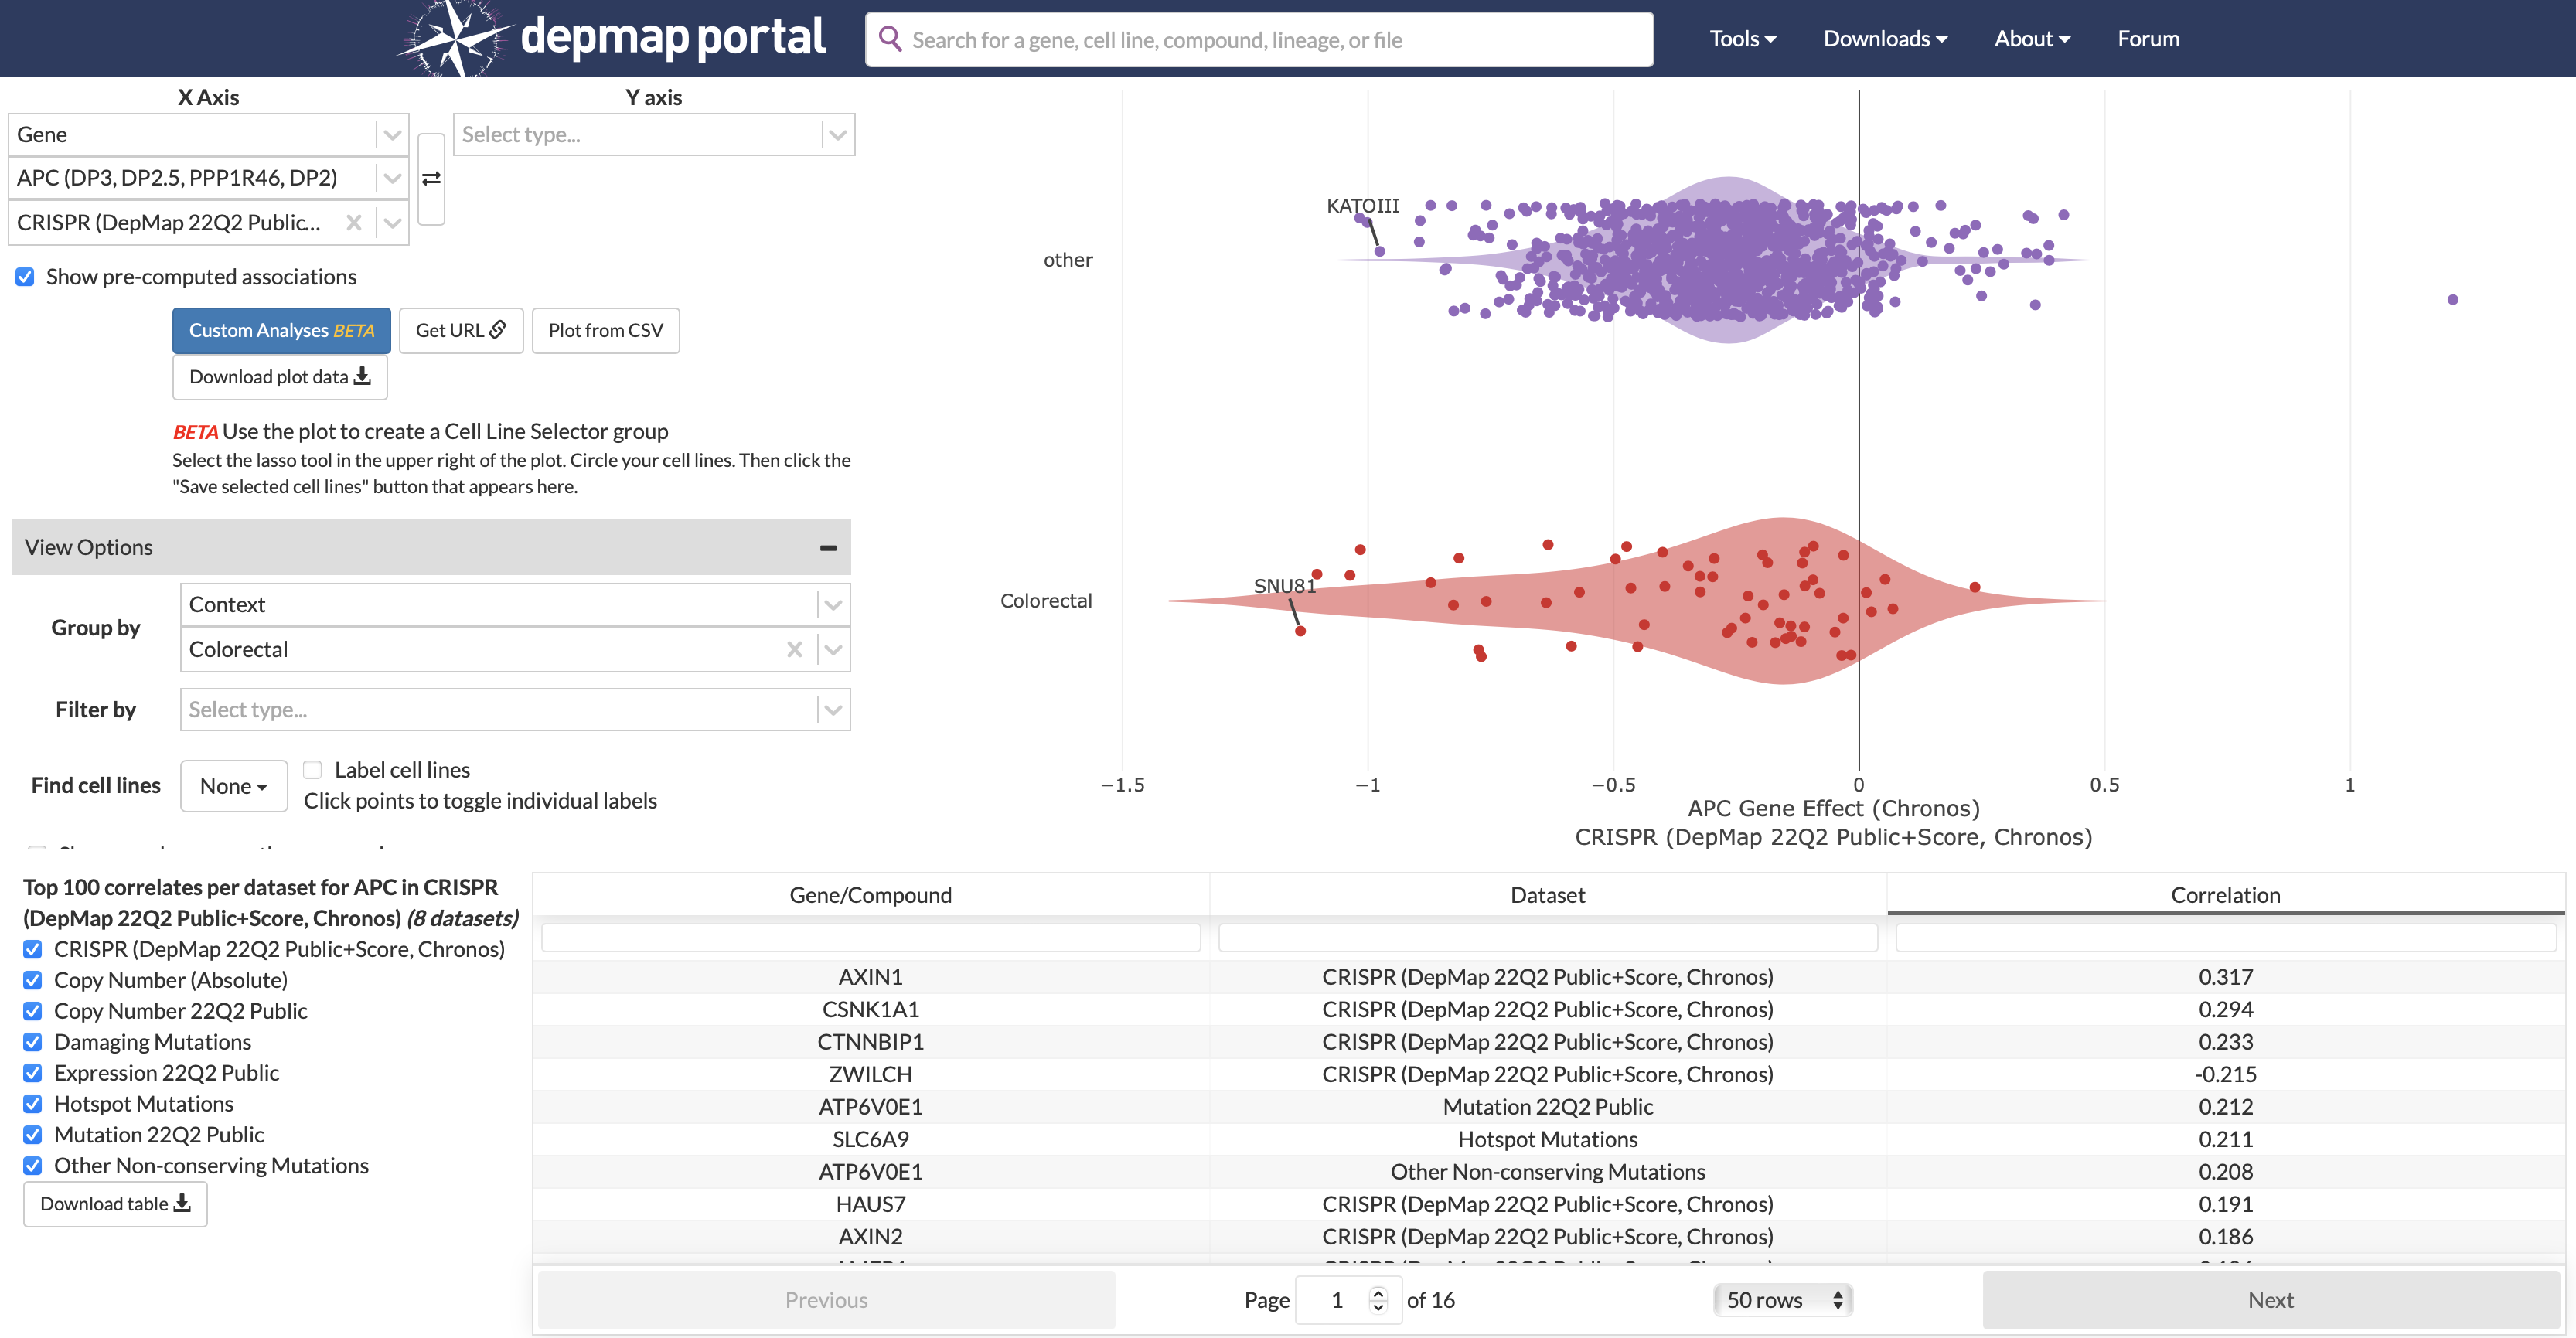
\includegraphics[width=\textwidth]{figures/Depmap_explorer_screenshot.png}
\end{frame}

{
 \usebackgroundtemplate{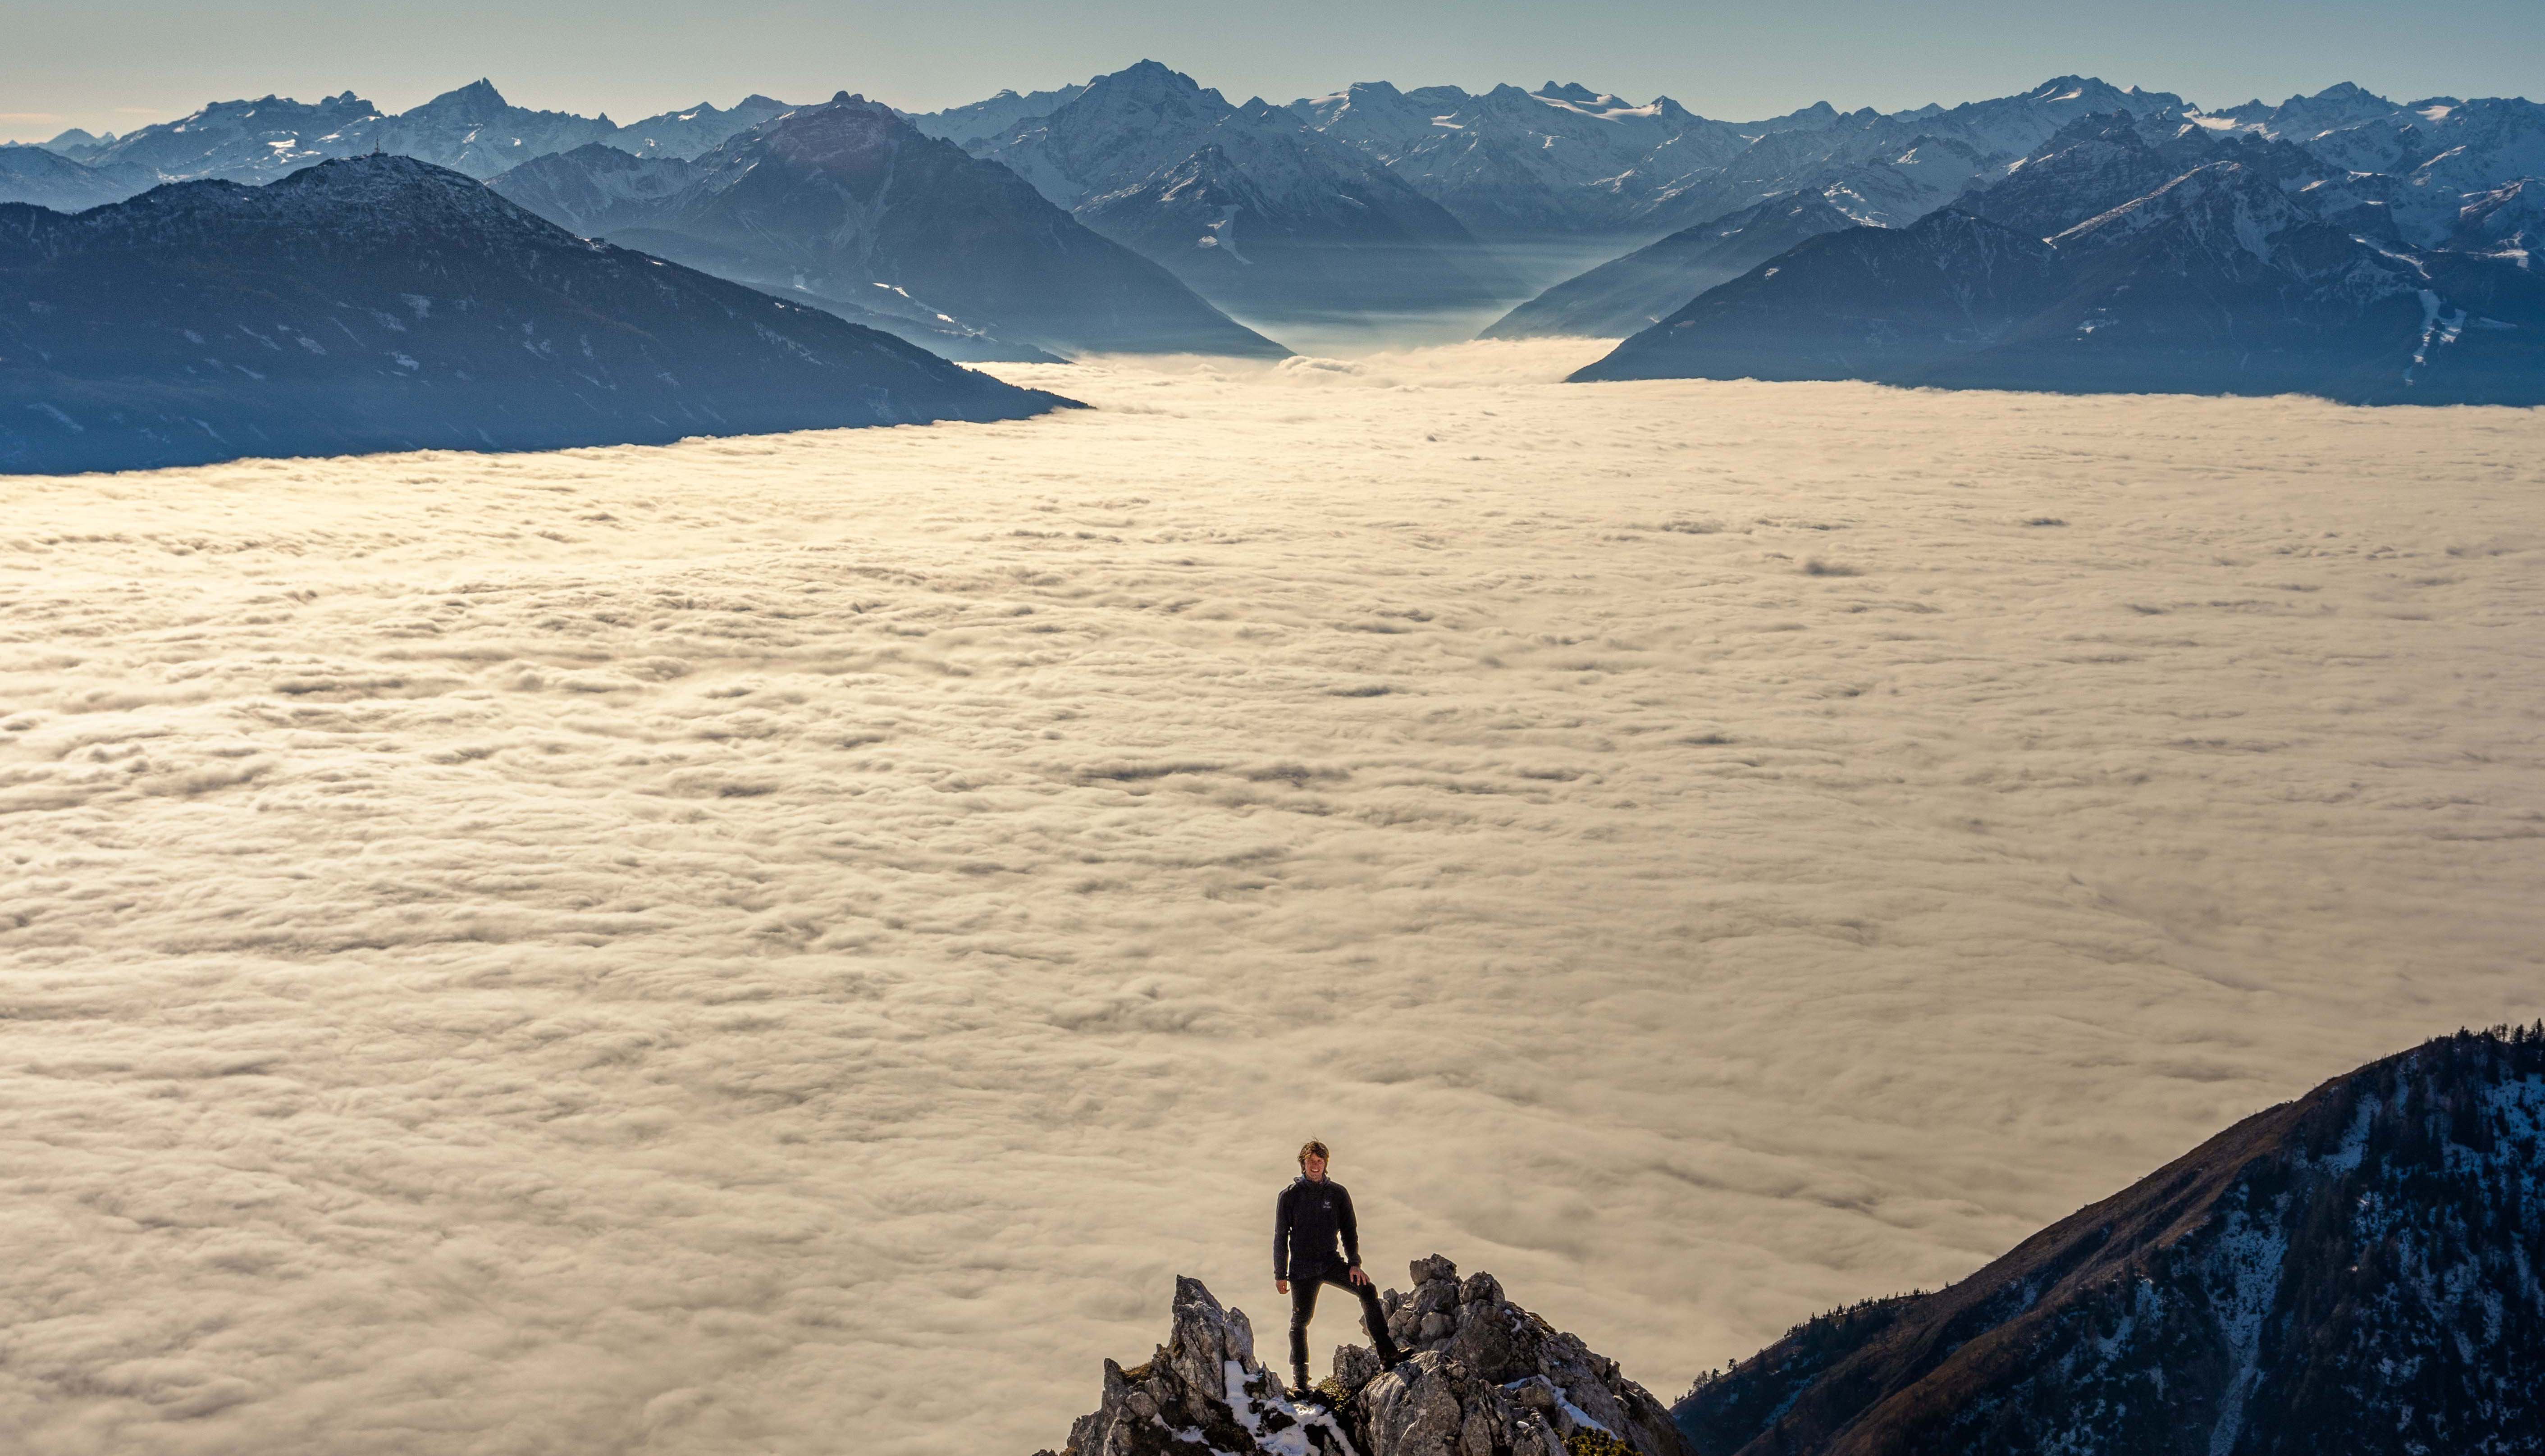
\includegraphics[width=\paperwidth]{figures/VJM_3542.jpg}}
  \begin{frame}
    \titlepage
  \end{frame}
}

\end{document}





